\documentclass{article}

% If you're new to LaTeX, here's some short tutorials:
% https://www.overleaf.com/learn/latex/Learn_LaTeX_in_30_minutes
% https://en.wikibooks.org/wiki/LaTeX/Basics

% Formatting
\usepackage[utf8]{inputenc}
\usepackage[margin=1in]{geometry}
\usepackage[titletoc,title]{appendix}
\usepackage{indentfirst}

% Math
% https://www.overleaf.com/learn/latex/Mathematical_expressions
% https://en.wikibooks.org/wiki/LaTeX/Mathematics
\usepackage{amsmath,amsfonts,amssymb,mathtools}

% Images
% https://www.overleaf.com/learn/latex/Inserting_Images
% https://en.wikibooks.org/wiki/LaTeX/Floats,_Figures_and_Captions
\usepackage{graphicx,float}

% Tables
% https://www.overleaf.com/learn/latex/Tables
% https://en.wikibooks.org/wiki/LaTeX/Tables

% Algorithms
% https://www.overleaf.com/learn/latex/algorithms
% https://en.wikibooks.org/wiki/LaTeX/Algorithms
\usepackage[ruled,vlined]{algorithm2e}
\usepackage{algorithmic}

% Code syntax highlighting
% https://www.overleaf.com/learn/latex/Code_Highlighting_with_minted
\usepackage{minted}
\usemintedstyle{borland}

% References
% https://www.overleaf.com/learn/latex/Bibliography_management_in_LaTeX
% https://en.wikibooks.org/wiki/LaTeX/Bibliography_Management
\usepackage{biblatex}
\addbibresource{references.bib}
\usepackage{graphicx}
\usepackage{placeins}

\title{Biol 461 Winter 2021 TA Section 02/26/21}
\author{}
\date{}

\begin{document}
\FloatBarrier

\maketitle
All Figures from Tsien et al. (1996)\cite{tsien_huerta_tonegawa_1996}:
\\
\\
\indent We have discussed how NMDA receptor channels (NMDARs) act as coincidence detectors, requiring both pre-synaptic and post-synaptic depolarization in order to open. Upon opening, NMDARs allow an influx of calcium, which can result in the recruitment of AMPA receptors to the synapse resulting in long-term potentiation.\\
\indent Researchers have long hypothesized that synaptic plasticity plays a role in memory storage. Researchers were interested in investigating whether NMDARs in the hippocampus (and potentially NMDAR mediated long-term potentiation) played a role in memory storage.  

\section{}
Several experiments were performed prior to the work of Tsien et al. suggesting that the disruption of NMDARs in the hippocampus resulted in deficient spatial learning in mice. \textbf{For each of the experiments described below, identify a weakness in the experimental design that results in the inability to fully attribute the deficiency in spatial learning to the hippocampal NMDARs.}
\begin{enumerate}
    \item Morris et al. (1986) infused rat brains with the NMDAR antagonist AP5, resulting in an elimination of hippocampal long-term-potentiation \cite{morris_1989}. These rats then became worse at a swim test in which they had to remember the location of a platform in a pool.
    \vspace{3.5cm}
    \item Silva et al. (1992) developed gene knockout mice that lacked a critical component of the calcium-calmodulin-dependent protein kinase II, which is a component of the NMDAR-activated cascade that results in long term potentiation. Mice with this knockout gene also lost their hippocampal long-term potentiation and became worse at the swim test \cite{silva_stevens_tonegawa_wang_1992}.
\end{enumerate}
\pagebreak
\section{}
Tsien et. al greated a gene knockout method that eliminated the expression of NMDARs in hippocampal CA1 cells (these mice are called CA1-KO mice). In situ hybridization of saggital slices of wild type and CA1-KO mice are shown in Figure 3 below.

\FloatBarrier
\begin{figure}[h]
  \centering
    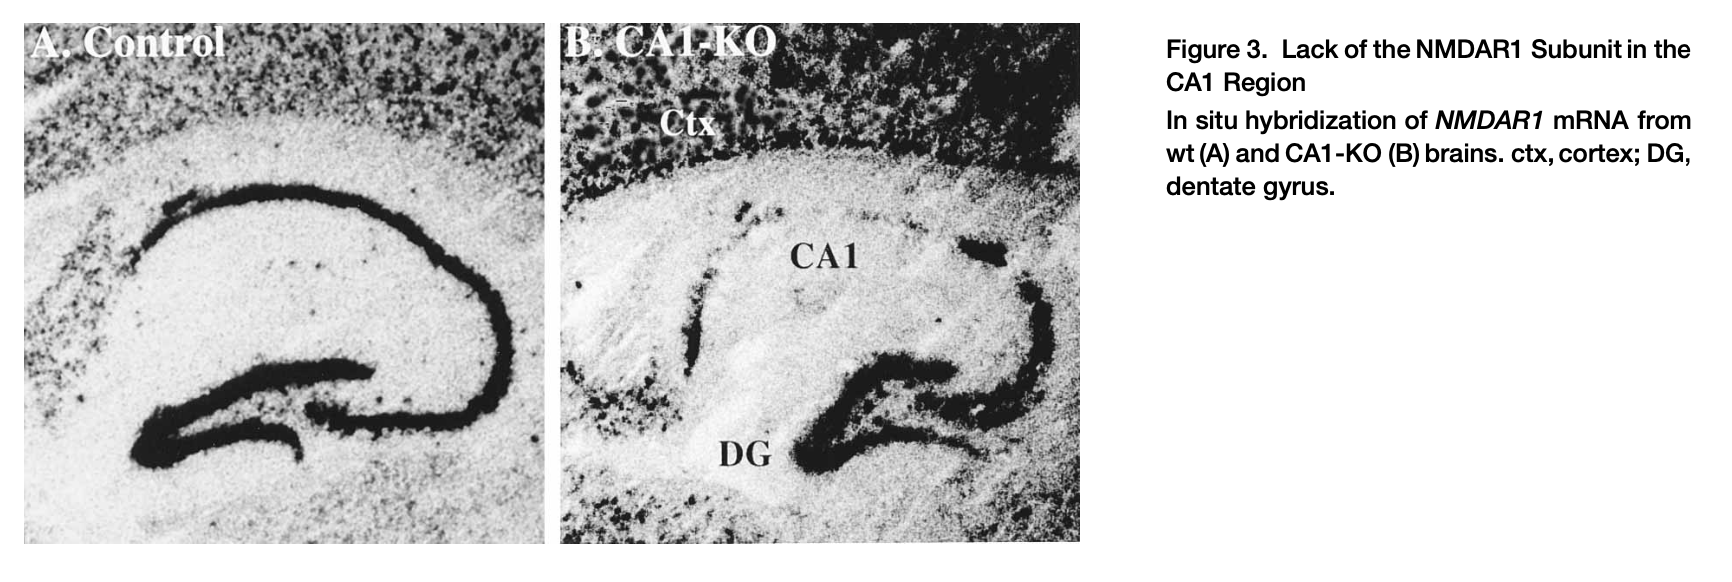
\includegraphics[width=.99\textwidth]{fig3.png}
\end{figure}
\FloatBarrier

These mice were then tested with the water maze.
\textbf{How does this experimental design avoid the weaknesses of the experiments described in part 1?}

\vspace{2cm}

\pagebreak
\section{}
There are a few versions of the swim test. In one (called the "hidden platform" test), there is a large, deep, round container of water. Somewhere in the container (hidden beneath the water) there is a platform where the mice can stand. The location of this platform is fixed. Researchers put the mice in the container on the platform to show them the location of the platform. Then, researchers put the mice in the water not on the platform and measure the time it takes for the mice to find the platform (mice do not like swimming).\\
\indent In another version of this test (called the "Landmark Task"), the setup is the same as above but three rectangular drawings are placed on the walls of the container, giving the mice the opportunity to associate the location of the platform with visual cues.\\
\indent The performance of the CA1-KO mice and control mice in both swim tests is shown in Figure 7 below
\FloatBarrier
\begin{figure}[h]
  \centering
    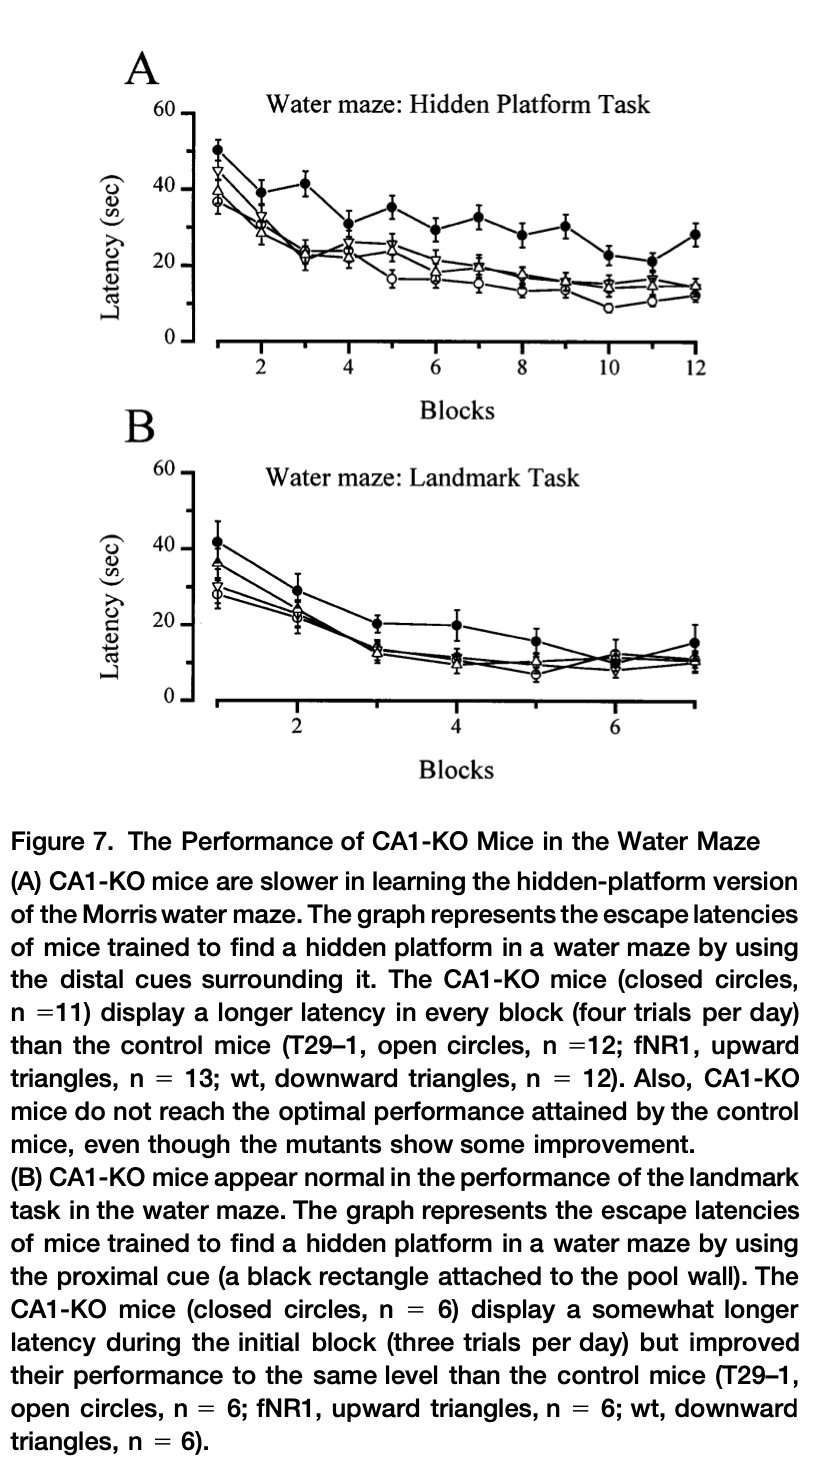
\includegraphics[width=.5\textwidth]{fig7.png}
\end{figure}
\FloatBarrier

\noindent \textbf{How do the performances of the CA1-KO mice and the wild type mice compare on the first and last trials of each swim test? What does this suggest aboout the spatial memory of the CA1-KO mice in comparison to the wild type mice?}

\pagebreak
Occasionally the mice were put in the pool in the Hidden Platform conditions for 60 seconds but the platform was removed (this is called the "Transfer Test". Figure 8c below shows three-dimensional graphs representing the total occupancy by six T29–1 mice and six CA1-KO mice during the last transfer test. 
\FloatBarrier
\begin{figure}[h]
  \centering
    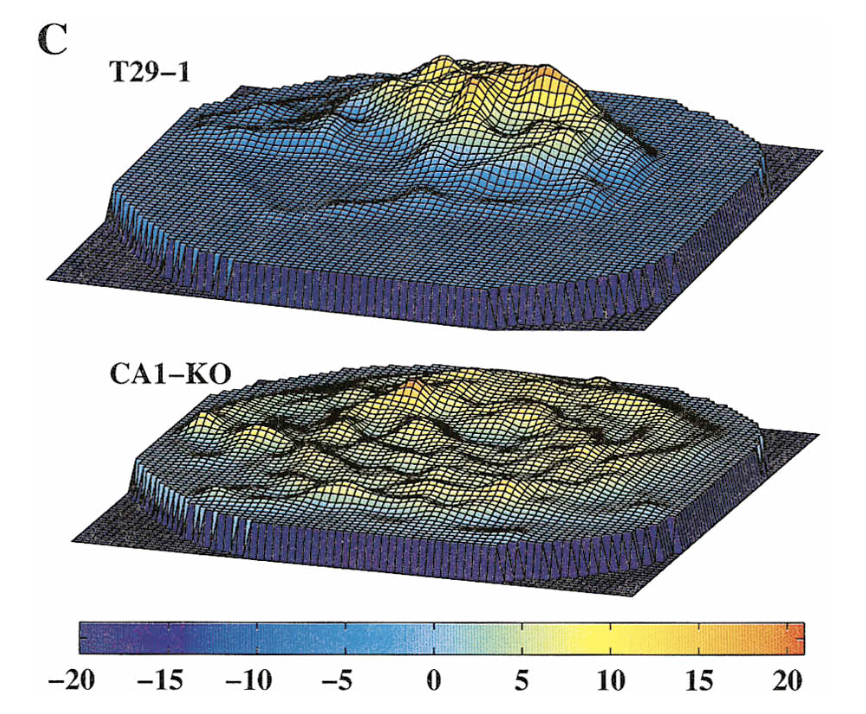
\includegraphics[width=.6\textwidth]{fig8c.png}
\end{figure}
\FloatBarrier

\noindent \textbf{How do the behaviors of the CA1-KO mice and control mice differ? What does this suggest about the spatial memories of each?}
\vspace{5cm}

\printbibliography
\end{document}
